%============================== Setting teh Document=============================================

\documentclass[aspectratio=169]{beamer}
\usepackage[english]{babel} 
\usepackage[utf8]{inputenc} 
\usepackage[T1]{fontenc}
\usepackage{graphicx}
\usepackage{xcolor}
\usetheme{AnnArbor}
\usepackage{multicol}
\usepackage[pscoord]{eso-pic}
\usepackage{tikz}
%==========================Set the foot line========================================================

\setbeamercolor*{author in head/foot}{parent=palette tertiary}
\setbeamercolor*{title in head/foot}{parent=palette primary}
\setbeamercolor*{date in head/foot}{parent=palette primary}

\defbeamertemplate*{footline}{}
{
	\leavevmode
	\hbox{%
		\begin{beamercolorbox}[wd=.25\paperwidth,ht=2.25ex,dp=1ex,center]{author in head/foot}%
			\usebeamerfont{author in head/foot}\centering{Telephone Number}
		\end{beamercolorbox}%
	
		\begin{beamercolorbox}[wd=.25\paperwidth,ht=2.25ex,dp=1ex,center]{title in head/foot}
			\usebeamerfont{title in head/foot}\centering{Mobile Number}
		\end{beamercolorbox}%
	
	        \begin{beamercolorbox}[wd=.25\paperwidth,ht=2.25ex,dp=1ex,center]{author in head/foot}%
	   	 	\usebeamerfont{author in head/foot}\centering{\href{mailto:f.rombaldoni@campus.uniurb.it}{f.rombaldoni@campus.uniurb.it}}
    	        \end{beamercolorbox}%

		\begin{beamercolorbox}[wd=.25\paperwidth,ht=2.25ex,dp=1ex,center]{date in head/foot}%
			\usebeamerfont{date in head/foot}\centering{Francesco Rombaldoni}\hspace*{2em}
		\end{beamercolorbox}}%
}
\AddToShipoutPictureFG{
	\put(\LenToUnit{.884\paperwidth},
	\LenToUnit{.25\paperheight})
	{\vtop{{\null}
	\makebox{\begin{tikzpicture}
	\clip (0,0) circle (6mm) node {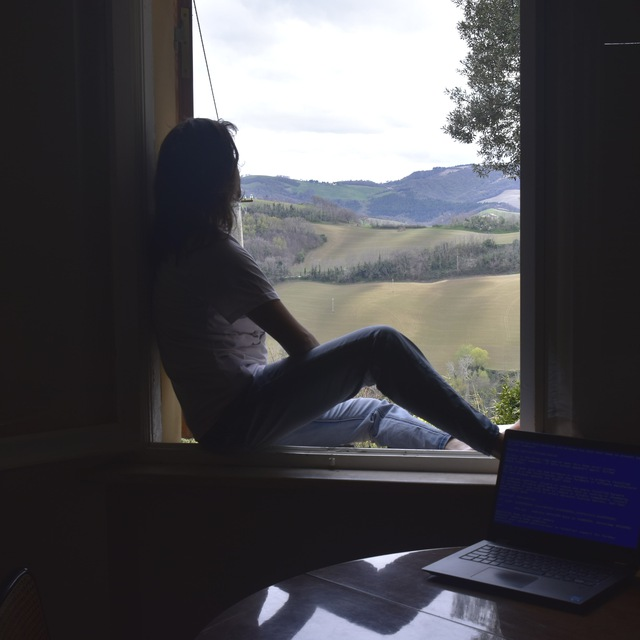
\includegraphics[width=22mm]{Imgs/temp}};
	\end{tikzpicture}}}}} 

%===========================================Document starting===============================================
\begin{document}

\section{Something}
\setbeamertemplate{navigation symbols}{}
\begin{frame}[t]{\textbf{Private Lessons Announcement}}
	
	\mbox{
	\colorbox{gray!20}{\begin{minipage}[t][0.8\textheight][t]
			{\dimexpr0.4\textwidth-2\fboxsep-2\fboxrule-5pt\relax}
			\centering{Private Lessons Announcemen text...}
	\end{minipage}}
		\colorbox{gray!20}{\begin{minipage}[t][0.8\textheight][t]
			{\dimexpr0.4\textwidth-2\fboxsep-2\fboxrule-5pt\relax}
		\textbf{Scientific Subject:}
		\begin{multicols}{2}
		\begin{itemize}
		\item Math
		\item Geometry
		\item Physics
		\item Science
		\end{itemize}
		\end{multicols}
		\textbf{Programming Languages:}
		\begin{multicols}{2}
		\begin{itemize}
			\item C
			\item C++
			\item C\#
			\item Java
			\item Prolog
			\item Haskell
			\item Python
			\item \LaTeX
			\item MarkDown
			\item HTML
			\item CSS
		\end{itemize}
		\end{multicols}
	\end{minipage}}


\colorbox{gray!20}{\begin{minipage}[t][0.8\textheight][t]
		{\dimexpr0.22\textwidth-2\fboxsep-2\fboxrule-5pt\relax}
		\centering{\textbf{Contact me on WhatsApp}}
			\begin{figure}
			\centering
			
\includegraphics[width=0.5\textwidth]{Imgs/WhatsApp-QR-code}
		\end{figure}
		\centering{\textbf{Contact me on Telegram}}
	\begin{figure}
		\centering
		
\includegraphics[width=0.5\textwidth]{Imgs/WhatsApp-QR-code}
	\end{figure}
	\end{minipage}}
}


\end{frame}

\end{document}
